\newpage
\section{Implementazione}
In questa sezione vengono analizzati gli aspetti implementativi del sistema, facendo eventualmente riferimento al codice
sviluppato. Nello specifico, verranno approfonditi solamente gli elementi che non sono stati esplorati a pieno nella
sezione Design di Dettaglio o che si ritengono fondamentali nello sviluppo di un progetto di tipo "game" come quello in
discussione.


\subsection{Marcantoni}
Il mio compito all'interno del progetto è stato quello di realizzare il \texttt{GameLoop}, i palloncini (l'entità base,
i vari "potenziamenti" e infine il rispettivo attore), la gestione dei round (con relativa DSL per la loro creazione e
l'attore che si occupa dello \textit{spawn} dei palloncini) e la suddivisione della logica del model nei tre
\textit{manager}. Ho inoltre collaborato con gli altri membri del team durante la fase di design delle entità.

\subsubsection{Game Loop}
Il \textit{game loop} è il ciclo infinito che si occupa di aggiornare il \texttt{Model} ed ordinare il conseguente
\textit{refresh} della \texttt{View}. Solitamente esso viene implementato mediante un ciclo \texttt{while(true)} ma,
avendo adottato il paradigma ad attori, ciò comporterebbe l'esecuzione di un \textit{handler} bloccante con
conseguente perdita totale di reattività da parte dell'attore \texttt{GameLoop}.

Tale effetto è stato evitato mediante un comportamento che sfrutta un \textit{timer}: l'attore \texttt{GameLoop} invia a
se stesso dei messaggi di tipo \texttt{Tick} distanziati tra loro da un \textit{delay} che dipende dal
\textit{frame rate} scelto per la partita. Alla ricezione di tale messaggio il \texttt{GameLoop} ordina al
\texttt{Model} di aggiornarsi; una volta ottenuta la risposta da quest'ultimo, ordina alla \texttt{View} di renderizzare
la lista di entità provenienti dal \texttt{Model}. Le interazioni appena descritte sono riportate in figura
\ref{fig:sequence-gameloop}.

\begin{figure}[H]
  \centering
  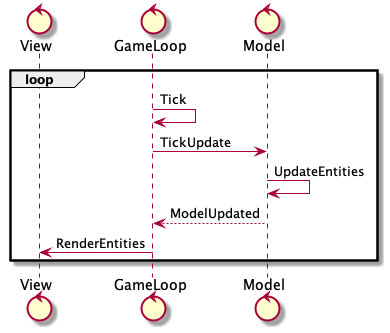
\includegraphics[width=.5\linewidth]{img/sequence-gameloop}
  \caption{Diagramma di sequenza delle interazioni del \texttt{GameLoop}.}
  \label{fig:sequence-gameloop}
\end{figure}

